\documentclass[a4paper,11pt]{article}
\usepackage[T1]{fontenc}
\usepackage[utf8]{inputenc}
\usepackage{lmodern}
\usepackage{graphicx}
\usepackage[hidelinks]{hyperref}

\title{User manual}
\author{FMC TDC Linux kernel support}
\date{}

\begin{document}

\maketitle
\tableofcontents

\newpage
\section{Introduction}

%\begin{figure}
  \begin{center}
    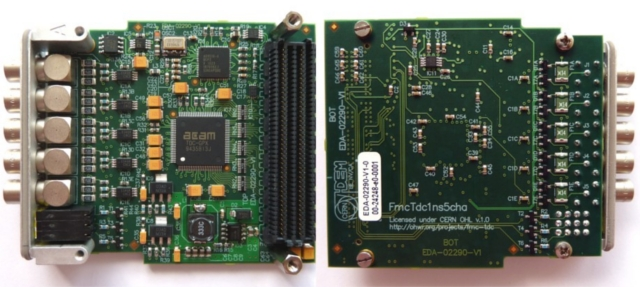
\includegraphics[scale=0.5]{img/fmc-tdc.jpg}
%    \label{fig:fmc-tdc}
%    \caption{FMC TDC board}
  \end{center}
%\end{figure}

$\newline$
In electronic instrumentation and signal processing, a time to digital converter (abbreviated TDC) is a device for recognizing events and providing a digital representation of the time they occurred. At this case, the FMC TDC outputs the time of arrival for each incoming pulse.

This is the project to provide support of the FMC TDC board in the Linux kernel plugged to a SPEC carrier board.

The aim is to provide an loadable module to be used along with this board for
the latest Linux kernel versions. The driver relies on ZIO framework and the FMC
bus dependencies, which are other projects hosted in OHWR.

\section{Installation}
\subsection{Dependencies}
To compile properly this driver, you should have downloaded the following repositories (branch master). For that purpose, you should have installed \textit{git} software. 
\begin{itemize}
  \item \href{http://www.ohwr.org/projects/zio}{ZIO} framework
  \item \href{http://www.ohwr.org/projects/spec-sw}{SPEC} driver
  \item \href{http://www.ohwr.org/projects/fmc-bus}{FMC bus} support
\end{itemize}

\subsection{Download the sources}

To download the sources, you should execute the following command:

\indent\indent\texttt{\$ git clone git://ohwr.org/fmc-projects/fmc-tdc/fmc-tdc-sw.git}

\subsection{Compile}

To compile the sources, you should execute the following command:

\indent\indent\texttt{\$ make}

\subsection{Load the drivers}

To load the drivers, we should load the dependencies first:

\indent\indent\texttt{\# insmod <path\_zio>/zio.ko} \\
\indent\indent\texttt{\# insmod <path\_fmc-bus>/kernel/fmc.ko} \\
\indent\indent\texttt{\# insmod <path\_spec-sw>/kernel/spec.ko} \\
Once the dependencies are loaded, we load the drivers:

\indent\indent\texttt{\# insmod <path\_fmc-tdc-sw>/drivers/spec-tdc.ko <parameters>} 

\subsubsection{FMC TDC driver parameters}

The spec-tdc.ko driver has several parameters, you can discover them executing: \texttt{modinfo ./spec-tdc.ko}.

\begin{itemize}
\item lun: Logical unit number.
\item bus: PCI bus number where the SPEC+TDC is plugged on.
\item slot: PCI slot where the SPEC+TDC is plugged on.
\end{itemize}

To know which are the bus and slot numbers, one can use the command \textit{lspci}:

\indent\indent\texttt{\$ lspci} \\
\indent\indent\texttt{[...]} \\
\indent\indent\texttt{00:04.0 Non-VGA unclassified device: CERN/ECP/EDU Device 018d (rev 03)} \\
In the previous output, the parameters will be: bus=0 slot=4.


\section{libtdc, an user-space library}

\subsection{Introduction}

To facilitate the task of managing the FMC TDC devices, it is provided an C/C++
user-space library. It is recommended to use it instead of accesing directly to
the driver.

\subsection{API}

\textbf{struct tdc\_board *tdc\_open(int lun);} \\
Open the selected device.\\
\textbf{int tdc\_close(struct tdc\_board *b);}  \\
Close the device. \\
\textbf{struct tdc\_time *tdc\_zalloc(unsigned int events);} \\
Allocate a struct tdc\_time buffer with \textit{events} number of events. \\
\textbf{void tdc\_free(struct tdc\_time *buffer);} \\
Free the previously allocated struct tdc\_time buffer. \\
\textbf{int tdc\_start\_acquisition(struct tdc\_board *b);} \\
Start acquisition.\\
\textbf{int tdc\_stop\_acquisition(struct tdc\_board *b);} \\
Stop acquisition.\\
\textbf{int tdc\_set\_host\_utc\_time(struct tdc\_board *b);} \\
Set FMC TDC time reference to local host UTC time. \\
\textbf{int tdc\_set\_utc\_time(struct tdc\_board *b, uint32\_t utc);} \\
Set FMC TDC time reference to a given value.\\
\textbf{int tdc\_get\_utc\_time(struct tdc\_board *b, uint32\_t *utc);} \\
Get FMC TDC time reference value. \\
\textbf{int tdc\_set\_dac\_word(struct tdc\_board *b, uint32\_t dw);} \\
Set FMC TDC DAC with a given value. \\
\textbf{int tdc\_get\_dac\_word(struct tdc\_board *b, uint32\_t *dw);} \\
Get FMC TDC DAC value. \\
\textbf{int tdc\_set\_time\_threshold(struct tdc\_board *b, uint32\_t thres);} \\
Set time threshold (time between IRQ where the event number acquired are less than the timestamp
threshold). In seconds. \\
\textbf{int tdc\_get\_time\_threshold(struct tdc\_board *b, uint32\_t *thres);} \\
Get time threshold.\\
\textbf{int tdc\_set\_timestamp\_threshold(struct tdc\_board *b, uint32\_t thres);} \\
Set timestamp threshold.\\
\textbf{int tdc\_get\_timestamp\_threshold(struct tdc\_board *b, uint32\_t *thres);} \\
Get timestamp threshold.\\
\textbf{int tdc\_set\_channels\_term(struct tdc\_board *b, uint32\_t config);} \\
Set channel termination resistor (50 Ohms). This is not an enable of the channel. \\
\textbf{int tdc\_get\_channels\_term(struct tdc\_board *b, uint32\_t *config);} \\
Get channel termination setup. \\
\textbf{int tdc\_activate\_channels(struct tdc\_board *b);} \\
Activate/enable all the channels to acquire data. This should be done before call tdc\_start\_acquisition(). \\
\textbf{int tdc\_deactivate\_channels(struct tdc\_board *b);} \\
Deactivate/disable all channels. \\
\textbf{int tdc\_get\_circular\_buffer\_pointer(struct tdc\_board *b, uint32\_t *ptr);} \\
Get circular buffer pointer value.\\
\textbf{int tdc\_clear\_dacapo\_flag(struct tdc\_board *b);} \\
Clear Dacapo flag from the circular buffer pointer value.\\
\textbf{int tdc\_read(struct tdc\_board *b, int chan, struct tdc\_time *t,
		    int n, int flags);} \\
Read \textit{n} events. The allowed flags are 0 (blocking read) or O\_NONBLOCK (non-blocking read).

\section{Test program}
\subsection{Introduction}
The test program is used to check the proper behavior of the board in case of failure or to check if there is a bug in the driver or in the library.

The test program has an CLI interface due to some limitations when accessing remotely to the machine. It is designed to allow the execution of the program under SSH.

\subsection{Dependencies}
\begin{itemize}
  \item Python 2.7 or higher.
\end{itemize}
First of all, you should compile the shared object library:

\indent\indent\texttt{\$ cd <path\_fmc-tdc-sw>/lib} \\
\indent\indent\texttt{\$ make libtdc.so}

\subsection{How to use it}

To execute it:

\indent\indent\texttt{\$ cd <path\_fmc-tdc-sw>/test} \\
\indent\indent\texttt{\$ sudo ./test-fmctdc.py} \\
If you want the help, you can execute:\\
\indent\indent\texttt{\$ ./test-fmctdc.py -h} \\

\section{Contact}
\href{http://www.ohwr.org/projects/fmc-tdc-sw}{FMC TDC Linux kernel support website} on \href{http://www.ohwr.org/}{OHWR}:

\indent\indent\texttt{\url{http://www.ohwr.org/projects/fmc-tdc-sw}}\\
\href{http://www.ohwr.org/mailing_list/show?project_id=fmc-tdc-sw}{Mailing list} on \href{http://www.ohwr.org/}{OHWR}:

\indent\indent\texttt{\url{http://www.ohwr.org/mailing_list/show?project_id=fmc-tdc-sw}}


\end{document}
